\documentclass[11pt]{article}
\usepackage[margin=1in]{geometry}
\usepackage{graphicx}
\usepackage{booktabs}
\usepackage{float}
\usepackage{listings}
\usepackage{xcolor}
\usepackage{hyperref}

\hypersetup{colorlinks=true, linkcolor=blue, urlcolor=blue, citecolor=blue}

\lstdefinestyle{pycode}{
  language=Python,
  basicstyle=\ttfamily\small,
  keywordstyle=\color{blue!70!black},
  commentstyle=\color{green!40!black},
  stringstyle=\color{orange!60!black},
  showstringspaces=false,
  frame=single,
  breaklines=true,
  tabsize=2
}

\title{Benchmarking Load Balancing Algorithms\\\large Greedy vs Local Search vs Genetic}
\author{Auto-generated from notebook execution}
\date{\today}

\begin{document}
\maketitle

\section{Objective}
This report compares three load balancing algorithms on a synthetic scheduling dataset:
\textbf{Greedy (LPT)}, \textbf{Local Search}, and a \textbf{Genetic Algorithm}. We evaluate:
\begin{itemize}
  \item execution time,
  \item precision (exact match rate against the optimum),
  \item error rate (average relative error).
\end{itemize}
The charts in this report were extracted from the executed benchmarking pipeline derived from
\texttt{load\_balancing\_benchmark.ipynb}.

\section{Experimental Setup}
\begin{itemize}
  \item Number of generated samples: 1000
  \item Tasks per sample: 12
  \item Number of servers: 3
  \item Test subset size: 200 (stratified by difficulty quantiles)
  \item Random seed: 42
\end{itemize}

\subsection*{Dataset Statistics}
\begin{table}[H]
\centering
\begin{tabular}{lr}
\toprule
Metric & Value \\
\midrule
Samples & 1000.0 \\
Tasks per sample & 12.0 \\
Servers & 3.0 \\
Mean total load & 552.741 \\
Std total load & 93.855 \\
Mean difficulty & 1.0336 \\
\bottomrule
\end{tabular}
\caption{Global dataset properties.}
\end{table}

\subsection*{Test Subset Distribution}
\begin{table}[H]
\centering
\begin{tabular}{cc}
\toprule
Difficulty bin & Count \\
\midrule
0 & 40 \\
1 & 40 \\
2 & 40 \\
3 & 40 \\
4 & 40 \\
\bottomrule
\end{tabular}
\caption{Stratified test subset (balanced across difficulty levels).}
\end{table}

\section{Visual Exploration}
\begin{figure}[H]
  \centering
  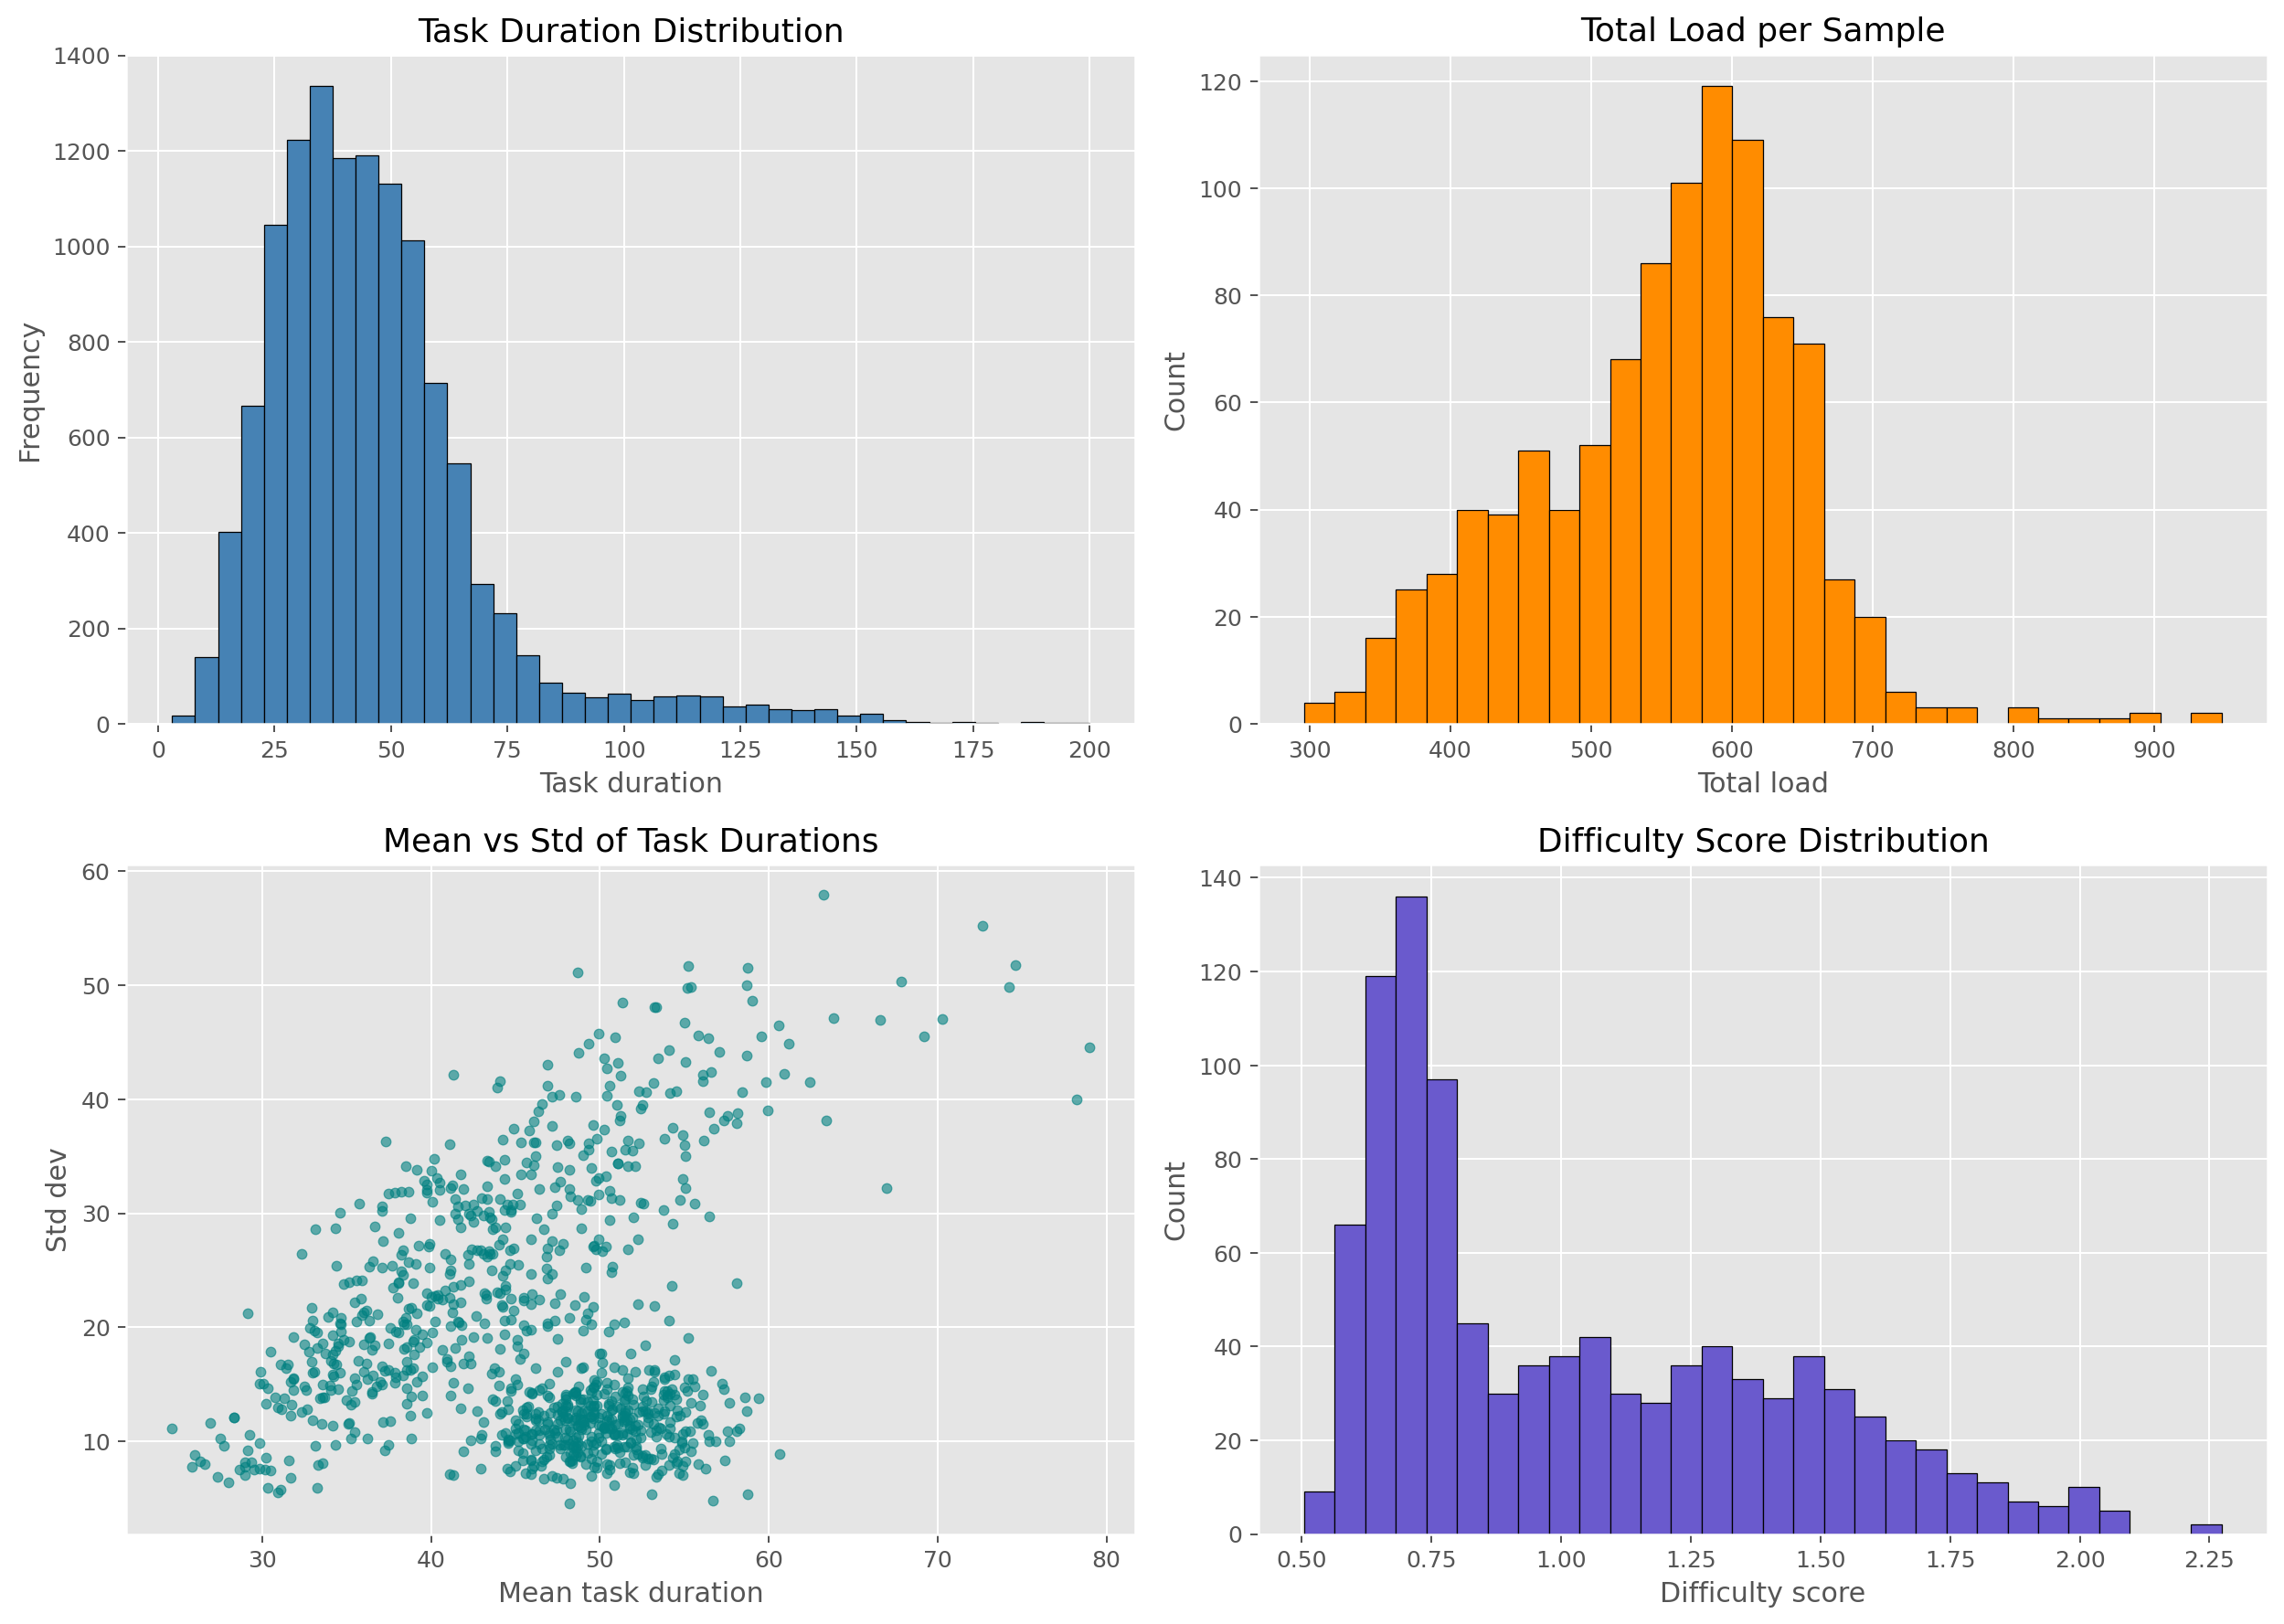
\includegraphics[width=0.95\textwidth]{report_assets/dataset_overview.png}
  \caption{Dataset overview: task duration distribution, total load, variance structure, and difficulty score.}
\end{figure}

\begin{figure}[H]
  \centering
  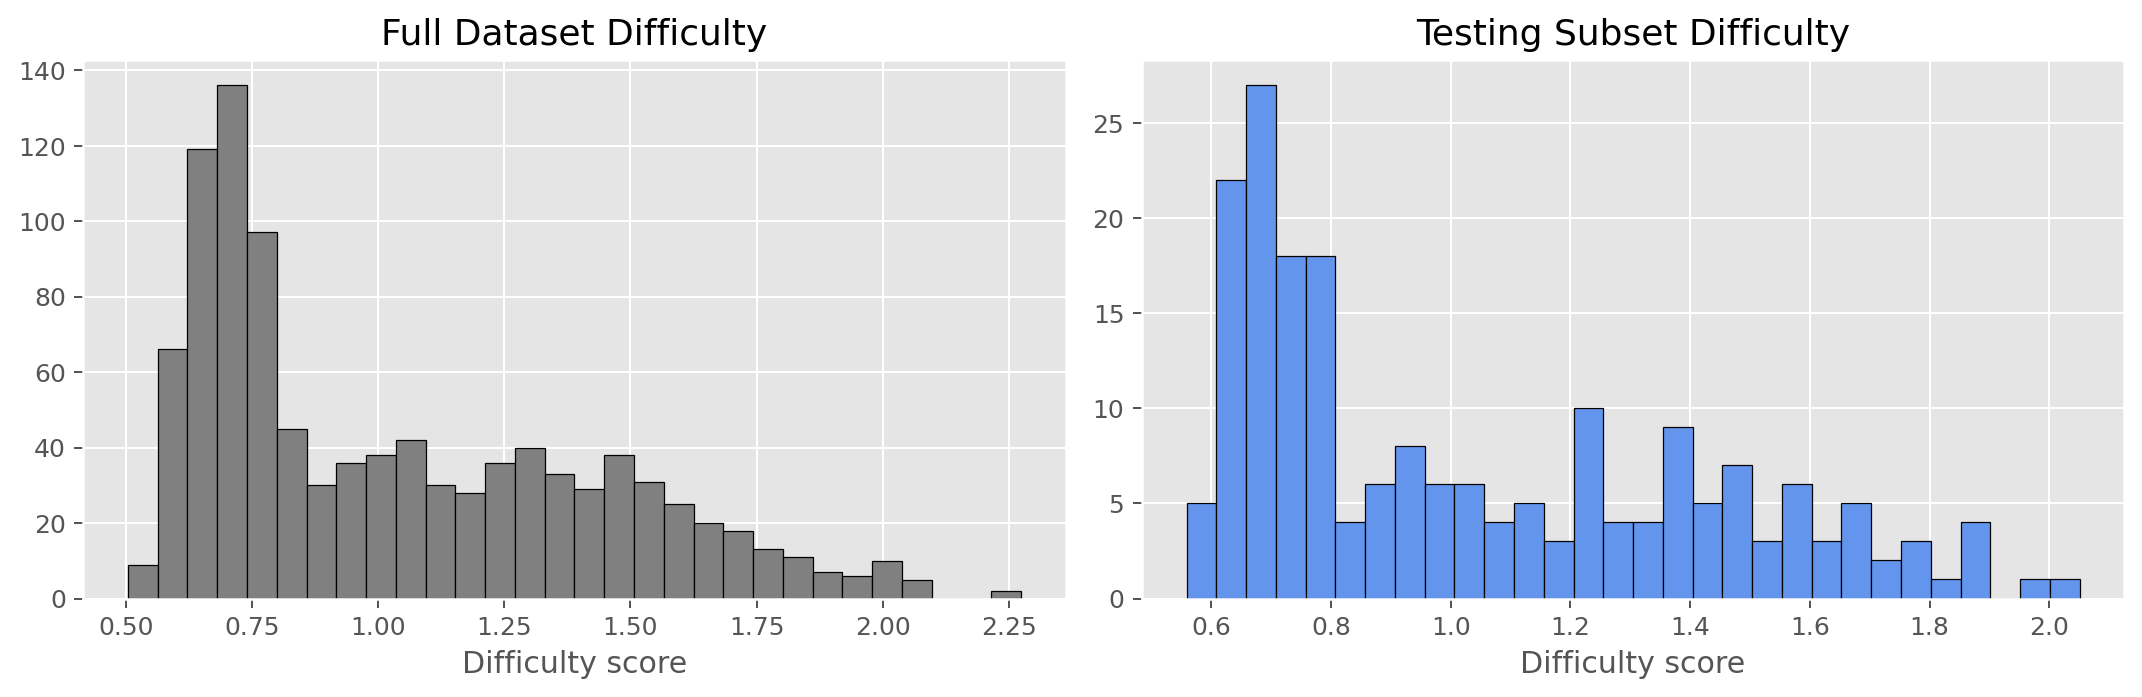
\includegraphics[width=0.85\textwidth]{report_assets/test_subset_difficulty.png}
  \caption{Difficulty distribution in full dataset vs stratified test subset.}
\end{figure}

\section{Algorithm Benchmark Results}
\begin{table}[H]
\centering
\begin{tabular}{lrrrrr}
\toprule
Algorithm & Avg runtime (ms) & Median runtime (ms) & Precision (\%) & Error rate (\%) & Worst error (\%) \\
\midrule
Genetic & 37.9103 & 36.0120 & 26.0 & 0.7998 & 3.5503 \\
Greedy (LPT) & 0.0162 & 0.0145 & 9.0 & 2.1878 & 8.4848 \\
Local Search & 0.2418 & 0.2269 & 38.0 & 0.6299 & 4.3750 \\
\bottomrule
\end{tabular}
\caption{Performance summary over 200 test instances.}
\end{table}

\begin{figure}[H]
  \centering
  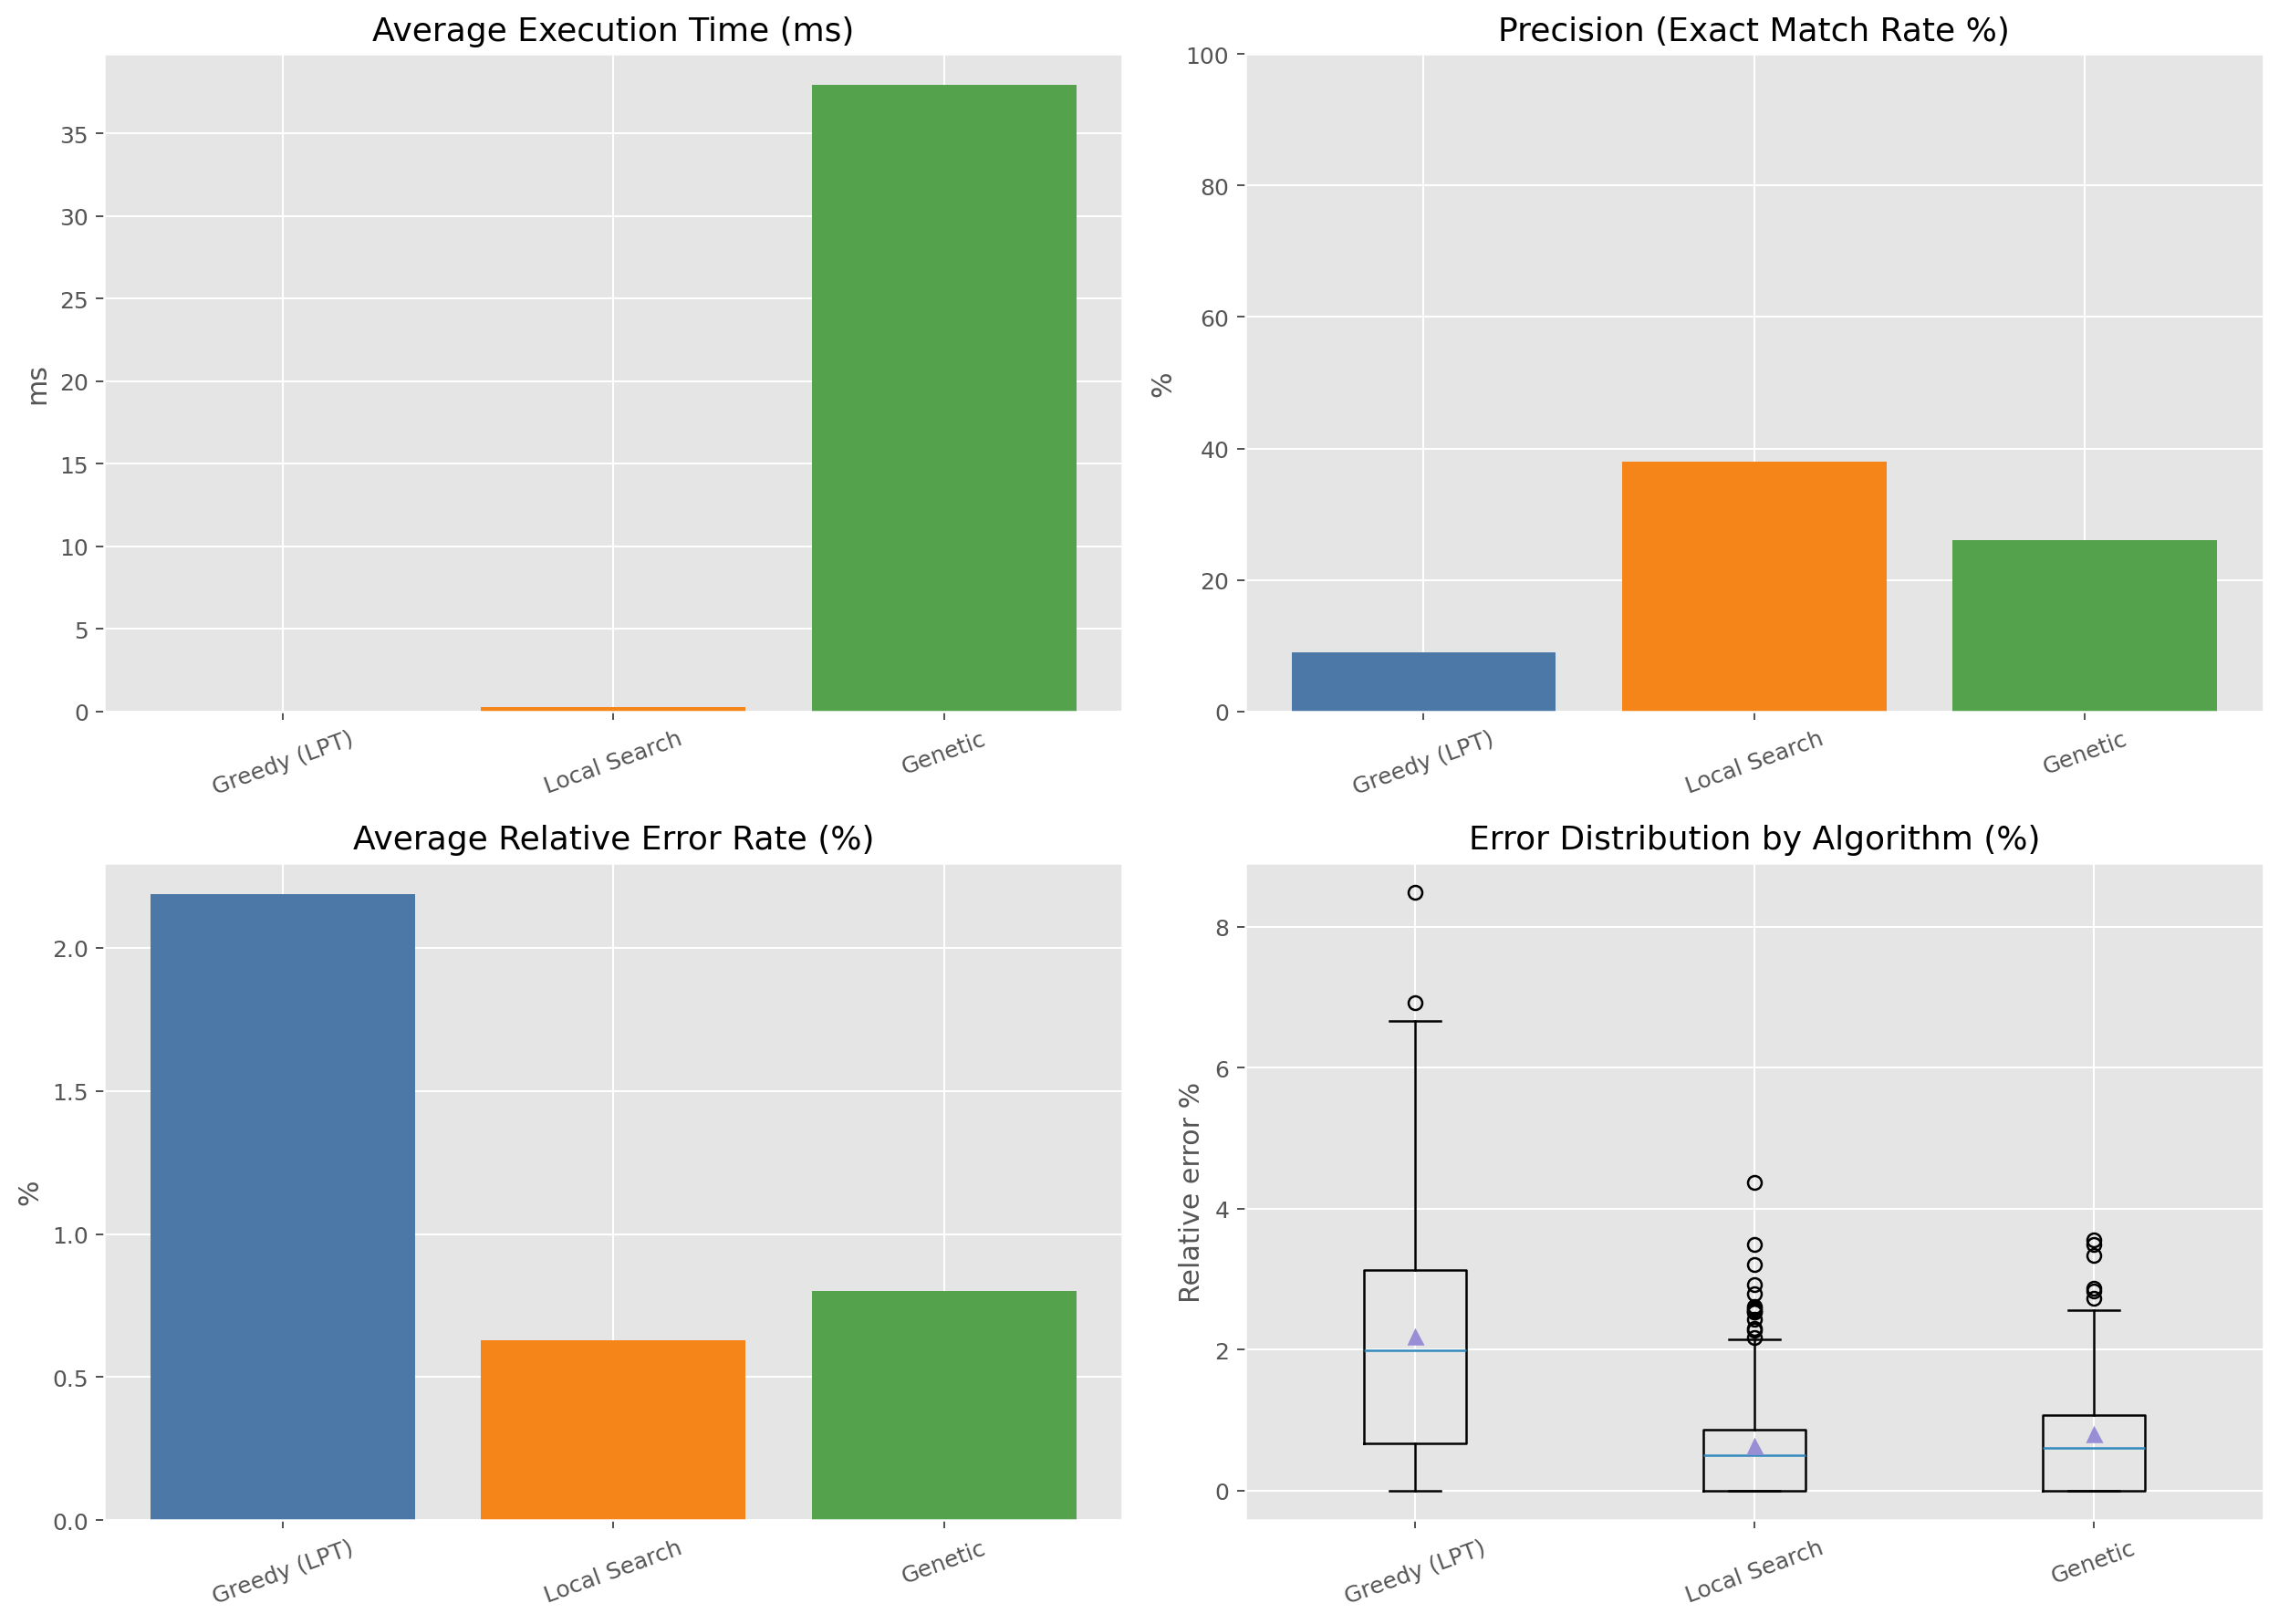
\includegraphics[width=0.95\textwidth]{report_assets/algorithm_comparison.png}
  \caption{Main comparison charts: runtime, precision, average error, and error distribution.}
\end{figure}

\begin{figure}[H]
  \centering
  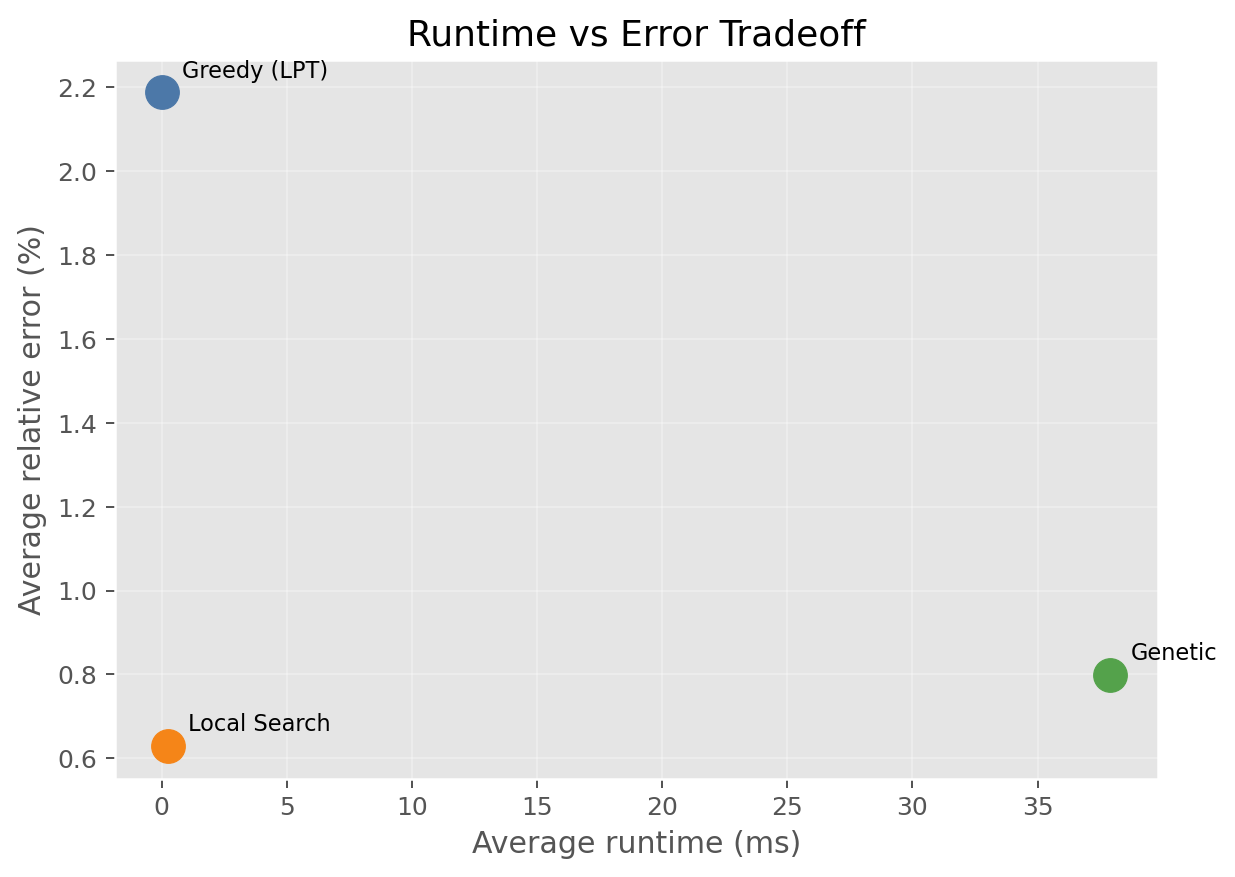
\includegraphics[width=0.70\textwidth]{report_assets/runtime_vs_error.png}
  \caption{Runtime vs error tradeoff for the three algorithms.}
\end{figure}

\section{Code Snippets (Minimal)}
\textbf{Snippet 1: Greedy baseline (LPT)}
\begin{lstlisting}[style=pycode]
def greedy_lpt(tasks, m=3):
    order = np.argsort(tasks)[::-1]
    loads = np.zeros(m, dtype=int)
    assignment = np.zeros(len(tasks), dtype=int)
    for i in order:
        s = int(np.argmin(loads))
        loads[s] += int(tasks[i])
        assignment[i] = s
    return int(loads.max()), assignment
\end{lstlisting}

\textbf{Snippet 2: Metrics extraction}
\begin{lstlisting}[style=pycode]
results['abs_error'] = results['predicted'] - results['optimal']
results['rel_error'] = results['abs_error'] / results['optimal']
results['is_exact'] = (results['predicted'] == results['optimal']).astype(int)

summary = results.groupby('algorithm', as_index=False).agg(
    avg_runtime_ms=('runtime_ms', 'mean'),
    precision=('is_exact', 'mean'),
    error_rate=('rel_error', 'mean')
)
\end{lstlisting}

\section{Interpretation}
\begin{itemize}
  \item \textbf{Greedy (LPT)} is by far the fastest method, but it shows the lowest precision and highest average error.
  \item \textbf{Local Search} provides the best overall quality in this setup: highest precision and lowest average error, with modest runtime.
  \item \textbf{Genetic} improves quality over Greedy but is significantly slower than both alternatives with the chosen hyperparameters.
  \item The runtime-error chart confirms a clear tradeoff: near-instant runtime (Greedy) vs stronger assignment quality (Local Search/Genetic).
\end{itemize}

\section{Final Conclusion}
For this benchmark configuration, \textbf{Local Search} is the best balance between speed and solution quality.
Use \textbf{Greedy (LPT)} for strict real-time constraints and \textbf{Genetic} when further quality exploration is needed and higher latency is acceptable.

\appendix
\section{Sample Execution Rows}
\begin{table}[H]
\centering
\scriptsize
\begin{tabular}{r l r r r r r}
\toprule
Sample & Algorithm & Optimal & Predicted & Runtime (ms) & Abs error & Rel error (\%) \\
\midrule
5  & Greedy (LPT) & 132 & 140 & 0.0185 & 8  & 6.0606 \\
5  & Local Search & 132 & 135 & 0.3619 & 3  & 2.2727 \\
5  & Genetic & 132 & 134 & 42.1506 & 2 & 1.5152 \\
7  & Greedy (LPT) & 195 & 200 & 0.0345 & 5  & 2.5641 \\
7  & Local Search & 195 & 195 & 0.4051 & 0  & 0.0000 \\
7  & Genetic & 195 & 196 & 43.2046 & 1 & 0.5128 \\
\bottomrule
\end{tabular}
\caption{Representative execution rows from the benchmark output.}
\end{table}

\end{document}
